\section{Passive Filter}

\begin{tabular}{@{}ll@{}}
    $f_{3 \, \deci \bel}= f_g$  & Cut-Off-Frequency, Corner-Frequency \\
                                & Dämpfung von $3 \, \deci \bel$ (d.h. Amplitude wird mit $\frac{1}{\sqrt{2}}$ 'verstärkt'), Phase: $- 45 \degree$ \\
    $f_S$                       & Sampling-Frequenz (ADC, digitale Filter) \\
                                & \textrightarrow\ Alle Frequenzen über $\frac{f_S}{2}$ müssen unterdrückt werden \\
    UTF                         & Übertragungsfunktion $G(s)$
\end{tabular}


\subsection{Tiefpassfilter 1. Ordnung}

\begin{minipage}[c]{0.3\columnwidth}
    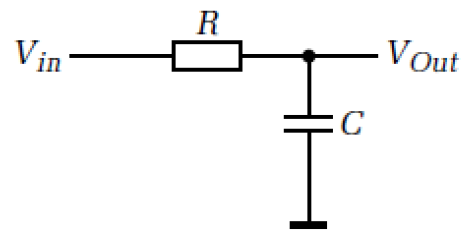
\includegraphics[width=\columnwidth]{images/tiefpass_ordnung_1.png}
\end{minipage}
\hfill
\begin{minipage}[c]{0.45\columnwidth}
    % $$ \text{UTF: } G(s) = \frac{V_{\rm out}}{V_{\rm in}} = \frac{\frac{1}{s \cdot C}}{R + \frac{1}{s \cdot C}} = \frac{1}{1 + s \cdot \underbrace{R \cdot C}_T} $$
    $$ \boxed{ G(s) = \frac{V_{\rm out}}{V_{\rm in}} = \frac{1}{1 + s \cdot \underbrace{R \cdot C}_T} } $$
\end{minipage}
\hfill
\begin{minipage}[c]{0.23\columnwidth}
    $$ \boxed{ f_{3 \, \deci \bel} = \frac{1}{2 \pi \underbrace{R C}_T} } $$
\end{minipage}

\textbf{Hinweis:} Die Zeitkonstante $T$ entspricht immer dem Parameter vor dem $s$. 
Beim Tiefpass 1. Ordnung entspricht dies $T = R \cdot C$


\subsection{Bodeplot Tiefpassfilter 1. und 2. Ordnung}

\begin{minipage}[t]{0.48\columnwidth}
    \begin{center}
        \myul{1. Ordnung}
    \end{center}
    \begin{itemize}
        \item Abfall von $- 20\, \deci \bel$ / Dekade
        \item Phasenschiebung von maximal $- 90 \degree$ (bei $f_g = -45 \degree$)
    \end{itemize}
\end{minipage}
\hfill
\begin{minipage}[t]{0.48\columnwidth}
    \begin{center}
        \myul{2. Ordnung}
    \end{center}
    \begin{itemize}
        \item Abfall von $- 40\, \deci \bel$ / Dekade
        \item Phasenschiebung von maximal $- 180 \degree$ (bei $f_g = -90 \degree$)
    \end{itemize}
\end{minipage}


\subsection{Filter 2. Ordnung}

\subsubsection{Kaskadierung von zwei gleichen Filtern}

\begin{minipage}[c]{0.48\columnwidth}
    $$ G_{11}(s) = \frac{1}{1 + s \cdot \underbrace{R \cdot C}_{T_2}} \cdot \frac{1}{1 + s \cdot \underbrace{R \cdot C}_{T_2}} $$
\end{minipage}
\hfill
\begin{minipage}[c]{0.48\columnwidth}
    $$ T_2 = \frac{\sqrt{\sqrt{2} - 1}}{2 \pi f_{3 \, \deci \bel} } \approx 0.64 \cdot T_1  $$
\end{minipage}

Daraus folgt, dass bei 2 identischen Stufen die Grenzfrequenz $f_{3 \, \deci \bel}$ der einzelnen Stufen $\frac{1}{0.64} = 1.56$ mal 
\textbf{höher} gewählt werden muss als bei einem Filter 1. Ordnung.


\subsubsection{Filter 2. Ordnung mit komplexen Polen}

\begin{minipage}[c]{0.6\columnwidth}
    $$ G(s) = \frac{A_0 \cdot p_1 \cdot p_2}{(p_1 + s) \cdot (p_2 + s)} = \frac{A_0 \cdot \omega_0^2}{s^2 + \frac{\omega_0}{Q} s + \omega_0^2} $$
$$ p_{1,2} = \frac{\omega_0}{2 Q} \big(1 \pm \sqrt{1 - 4 Q^2} \big) $$
\end{minipage}
\hfill
\begin{minipage}[c]{0.38\columnwidth}
    \begin{tabular}{ll}
        $p_i$       & Polstellen \\
                    & komplex für $Q > \frac{1}{2}$ \\
        $Q$         & Polgüte / Filtergüte \\
        $\omega_0$  & Polfrequenz
    \end{tabular}
\end{minipage}


% bei Platzmangel weglassen
\subsection{Filter höherer Ordnung}

\begin{itemize}
    \item Systeme höherer Ordnung können in kaskadierte Teilsysteme 1. \& 2. Ordnung aufgeteilt werden
    \item Höhere Ordnung und komplexe Pole ermöglichen steileren Übergang zwischen Durchlass- und Sperrbereich
\end{itemize}

Folgende Filter erzielen durch unterschiedliche Polverteilungen untersch. Verhalten:

\begin{itemize}
    \item \textbf{Butterworth:} Konstant im Durchlassbereich der UTF
    \item \textbf{Bessel:} Beste Rechteckübertragung, kein Überschwingen
    \item \textbf{Tschebyscheff:} Steilster Abfall im Sperrbereich der UTF
\end{itemize}


\subsection{Zeitverhalten: Schrittantwort}

\begin{enumerate}
    \item Frenqenzbereich: \textbf{Multiplikation} der UTF mit $\frac{1}{s}$
    \item Rücktransformation in den Zeitbereich, um $t_{\rm step}(t)$ zu erhalten
\end{enumerate}


\subsubsection{Tiefpass 1. Ordnung}

\begin{minipage}[c]{0.48\columnwidth}
    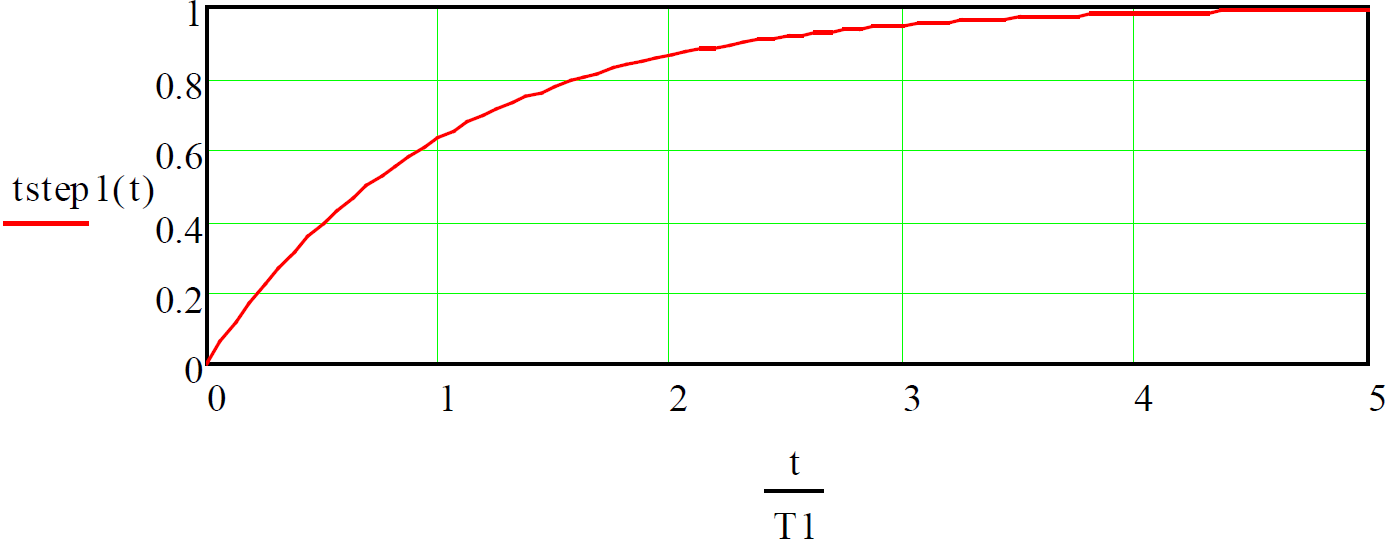
\includegraphics[width=\columnwidth]{images/schrittantwort_tp_ordnung_1.png}
\end{minipage}
\hfill
\begin{minipage}[c]{0.48\columnwidth}
    $$  t_{\rm step,1}(t) = 1 - e^{- \frac{t}{T_1}} $$
\end{minipage}


\subsubsection{Tiefpass 2. Ordnung}

\begin{minipage}[c]{0.43\columnwidth}
    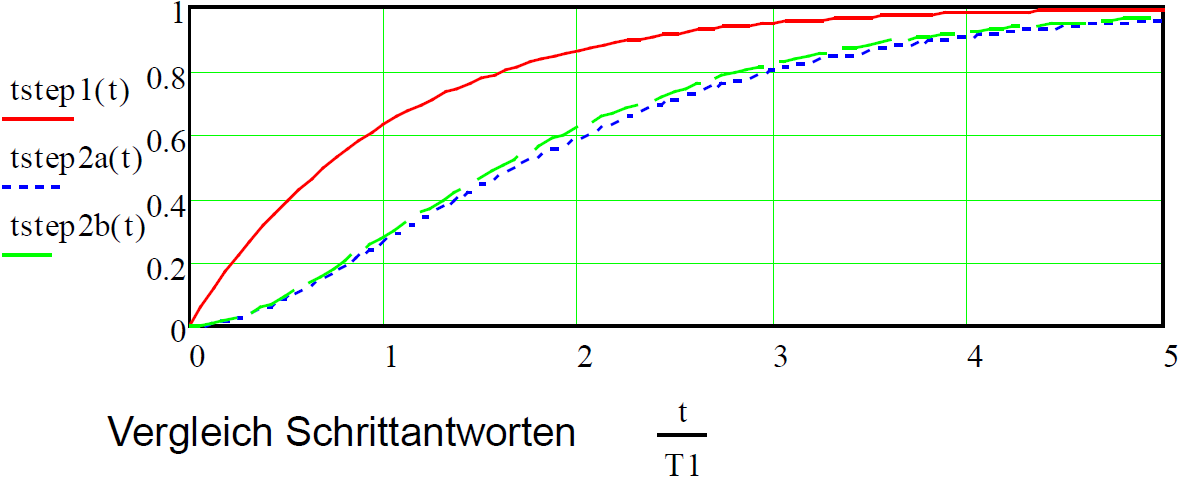
\includegraphics[width=\columnwidth]{images/schrittantworten_vergleich.png}
\end{minipage}
\hfill
\begin{minipage}[c]{0.55\columnwidth}
    $$ t_{\rm step2a}(t) = 1 - e^{- \frac{t}{T_1}}\cdot \left\lgroup 1 + \frac{t}{T_1} \right\rgroup $$
    $$ t_{\rm step2b}(t) = 1 - \left\lgroup \frac{T_1 \cdot e^{- \frac{t}{T_1}} - T_2 \cdot e^{- \frac{t}{T_2}}}{T_1 - T_2} \right\rgroup $$
\end{minipage}


\subsection{Schrittantworten verschiedener Polgüten}

\begin{minipage}[c]{0.48\columnwidth}
    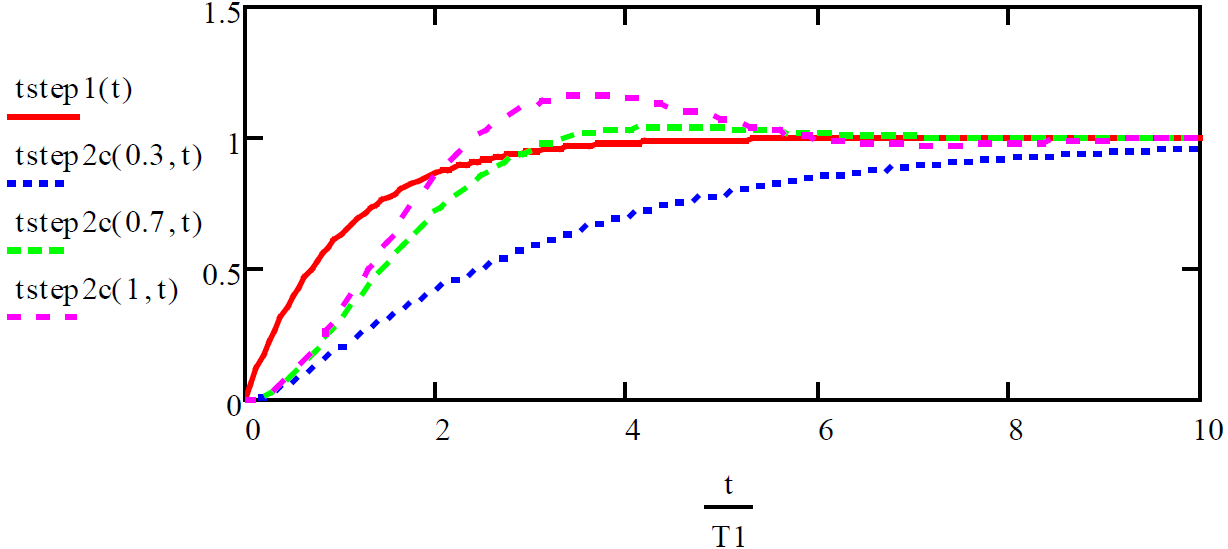
\includegraphics[width=\columnwidth]{images/schrittantwort_verschiedene_polgueten.png}
\end{minipage}
\hfill
\begin{minipage}[c]{0.48\columnwidth}
    Komplexe Pole ($Q > \frac{1}{2}$) führt zu Überschwingern. \\
    Bei einer Polgüte von $Q = \frac{1}{\sqrt{2}} \approx 0.7$ (\cgn{grüne Kurve}) schwingt das System am schnellsten ein!
\end{minipage}


\subsection{Filter 2. Ordnung (passiv und aktiv)}

% Allgmeingültig, egal ob aktive oder passive Filter
\begin{minipage}[c]{0.48\columnwidth}
    \begin{center}
        \myul{\textbf{Tiefpass}}
    \end{center}
    $$ \boxed{ G(s) = \frac{V_{\rm out}}{V_{\rm in}} = \frac{A_0}{\frac{1}{\omega_0^2} s^2 + \frac{1}{\omega_0 \cdot Q} s + 1 } } $$
\end{minipage}
\hfill
\begin{minipage}[c]{0.48\columnwidth}
    \begin{center}
        \myul{\textbf{Bandpass}}
    \end{center}
    $$ \boxed{ G(s) = \frac{V_{\rm out}}{V_{\rm in}} = \frac{\frac{A_0}{\omega_0 \cdot Q} s}{\frac{1}{\omega_0^2} s^2 +  \frac{1}{\omega_0 \cdot Q} s + 1 } } $$
\end{minipage}

\vspace{0.2cm}

\begin{minipage}[t]{0.48\columnwidth}
    \begin{center}
        \myul{\textbf{Hochpass}}
    \end{center}
    $$ \boxed{ G(s) = \frac{V_{\rm out}}{V_{\rm in}} = \frac{\frac{A_0}{\omega_0^2} s^2}{\frac{1}{\omega_0^2} s^2 + \frac{1}{\omega_0 \cdot Q} s + 1 } } $$
\end{minipage}
\hfill
\begin{minipage}[t]{0.48\columnwidth}
    \begin{center}
        \myul{\textbf{Aufbau Nenner}}
    \end{center}
    \begin{outline}
        \1 Alle Terme positiv
        \1 $s^2$-Term definiert Grenzfrequenz
        \1 Im $s$-Term ist Dämpfung enthalten
            \2 $s$-Term gross \textrightarrow\ grosse Dämpfung
            \2 $s$-Term $= 0$ \textrightarrow\ Oszillator!
    \end{outline}
\end{minipage}

\vspace{0.2cm}

Passive RC-Filter können maximal Güte $0.5$ haben (entkoppelte reelle Pole). Filter höherer Güte benötigen entweder
Spulen oder \textbf{Verstärker}. \\
\textbf{\textrightarrow\ Die Formeln gelten aber für passive und aktive Filter!}



\example{UTF Tiefpass 2. Ordnung}

\begin{minipage}[c]{0.4\columnwidth}
    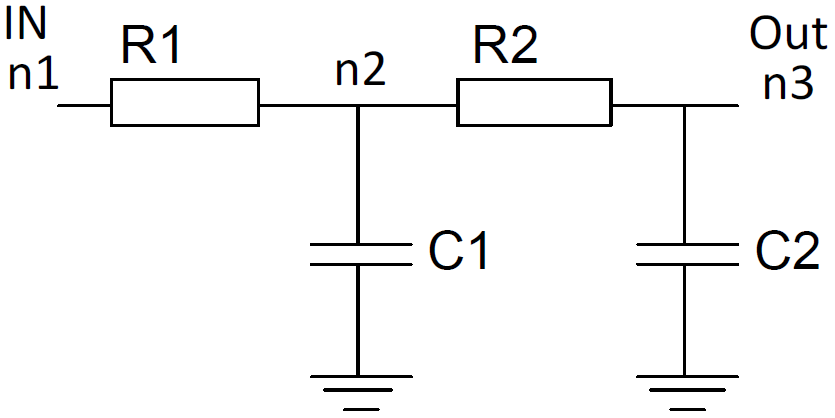
\includegraphics[width=\columnwidth]{images/tiefpass_ordnung_2.png}
\end{minipage}
\hfill
\begin{minipage}[c]{0.58\columnwidth}
    $$ A_0 = 1 \qquad \omega_0 = \frac{1}{\sqrt{C_1 C_2 R_1 R_2}} $$
    $$ Q = \frac{\sqrt{C_1 C_2 R_1 R_2}}{C_1 R_1 + C_2 R_1 + C_2 R_2} $$
\end{minipage}
$$ G(s) = \frac{V_{\rm out}}{V_{\rm in}} = \frac{1}{1 + (C_1 R_1 + C_2 R_1 + C_2 R_2) \cdot s + C_1 C_2 R_1 R_2 \cdot s^2 } $$

